\documentclass[border=15pt]{standalone}
\usepackage{tikz}
\usetikzlibrary{shapes.geometric, arrows.meta, positioning, calc, shadows.blur}

% Define colors
\definecolor{hardwaregray}{RGB}{127, 140, 141}
\definecolor{epicsblue}{RGB}{52, 73, 94}
\definecolor{blueskyorange}{RGB}{230, 126, 34}
\definecolor{ros2green}{RGB}{39, 174, 96}
\definecolor{moveitpurple}{RGB}{142, 68, 173}

\begin{document}
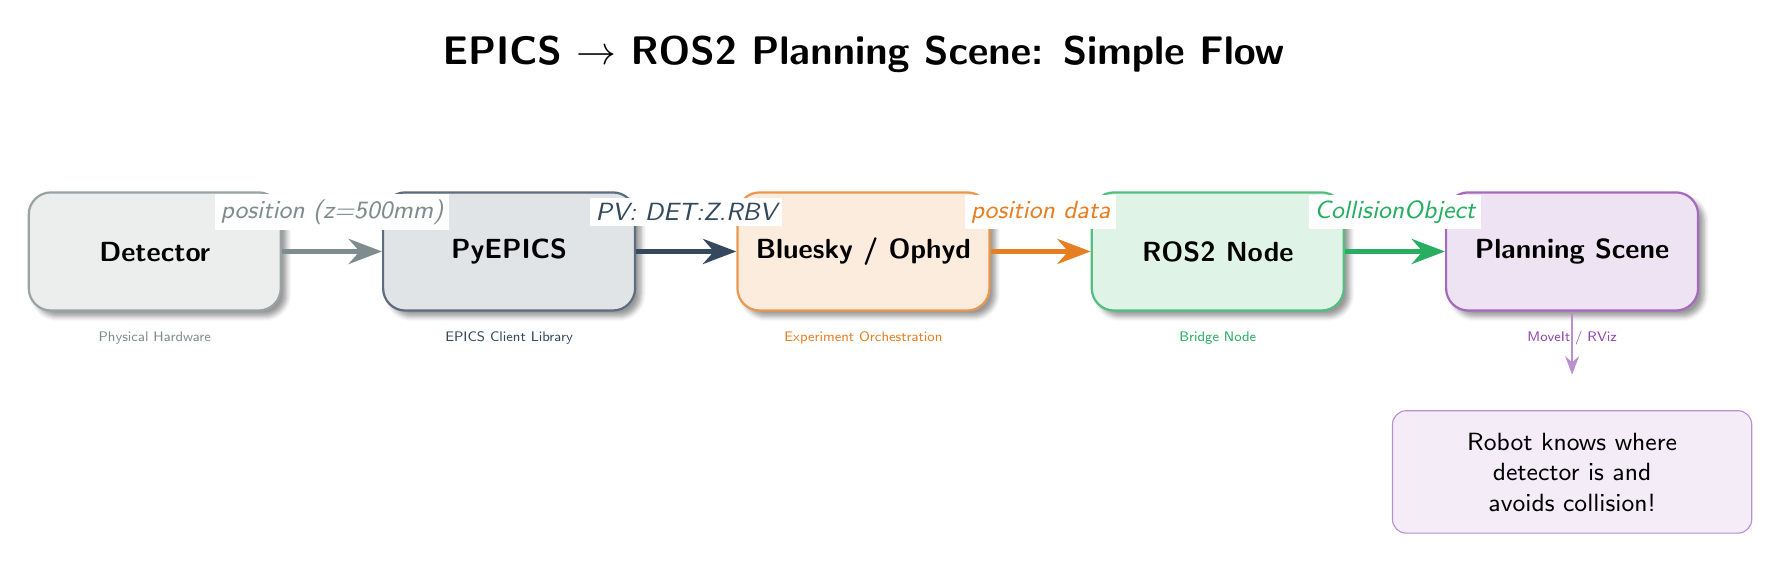
\begin{tikzpicture}[
    % Node styles
    block/.style={
        rectangle,
        rounded corners=8pt,
        draw=#1!80,
        fill=#1!15,
        thick,
        minimum width=3.2cm,
        minimum height=1.5cm,
        font=\sffamily\bfseries,
        blur shadow={shadow blur steps=5}
    },
    arrow/.style={
        ->,
        >=Stealth,
        line width=2pt,
        color=#1
    },
    datalabel/.style={
        font=\small\sffamily\itshape,
        color=#1,
        fill=white,
        inner sep=2pt
    }
]

% ============================================
% MAIN FLOW (Left to Right)
% ============================================

% 1. Hardware - Detector
\node[block=hardwaregray] (detector) at (0, 0) {Detector};
\node[font=\tiny\sffamily, color=hardwaregray] at (0, -1.1) {Physical Hardware};

% 2. PyEPICS
\node[block=epicsblue] (pyepics) at (4.5, 0) {PyEPICS};
\node[font=\tiny\sffamily, color=epicsblue] at (4.5, -1.1) {EPICS Client Library};

% 3. Bluesky/Ophyd
\node[block=blueskyorange] (bluesky) at (9, 0) {Bluesky / Ophyd};
\node[font=\tiny\sffamily, color=blueskyorange] at (9, -1.1) {Experiment Orchestration};

% 4. ROS2
\node[block=ros2green] (ros2) at (13.5, 0) {ROS2 Node};
\node[font=\tiny\sffamily, color=ros2green] at (13.5, -1.1) {Bridge Node};

% 5. Planning Scene
\node[block=moveitpurple] (planning) at (18, 0) {Planning Scene};
\node[font=\tiny\sffamily, color=moveitpurple] at (18, -1.1) {MoveIt / RViz};

% ============================================
% ARROWS WITH DATA LABELS
% ============================================

% Detector -> PyEPICS
\draw[arrow=hardwaregray] (detector.east) -- (pyepics.west);
\node[datalabel=hardwaregray] at (2.25, 0.5) {position (z=500mm)};

% PyEPICS -> Bluesky
\draw[arrow=epicsblue] (pyepics.east) -- (bluesky.west);
\node[datalabel=epicsblue] at (6.75, 0.5) {PV: DET:Z.RBV};

% Bluesky -> ROS2
\draw[arrow=blueskyorange] (bluesky.east) -- (ros2.west);
\node[datalabel=blueskyorange] at (11.25, 0.5) {position data};

% ROS2 -> Planning Scene
\draw[arrow=ros2green] (ros2.east) -- (planning.west);
\node[datalabel=ros2green] at (15.75, 0.5) {CollisionObject};

% ============================================
% TITLE
% ============================================
\node[font=\Large\sffamily\bfseries] at (9, 2.5) {EPICS $\rightarrow$ ROS2 Planning Scene: Simple Flow};

% ============================================
% RESULT ANNOTATION
% ============================================
\node[rectangle, rounded corners=5pt, draw=moveitpurple!60, fill=moveitpurple!10,
      text width=4cm, font=\small\sffamily, align=center, inner sep=8pt]
      at (18, -2.8) {
    Robot knows where\\detector is and\\avoids collision!
};
\draw[->, >=Stealth, thick, color=moveitpurple!60] (planning.south) -- ++(0, -0.8);

\end{tikzpicture}
\end{document}
